The results of Chapter~\ref{chap:within} are obtained under a \emph{within-subject} protocol: for
each participant, a model is trained on 280 of that participant's trials and tested
on the remaining 120. Limitation~2 of this thesis acknowledges that such figures
cannot support a generalisation claim. This chapter removes that limitation by
re-running the entire pipeline under a subject-disjoint protocol and reporting what
the system achieves on participants it has never seen.

\section{Motivation: What Within-Subject Evaluation Conceals}
\label{sec:cs_motivation}

Under the within-subject protocol, every encoder sees the test participant's face,
voice and neural signature during training. The reported accuracy therefore answers
the question \emph{``how well does the system recognise emotions in a person it has
already studied?''}, not \emph{``does the system recognise emotions?''}. For a
deployment scenario---clinical screening, human-computer interaction, or the
demonstration component of this thesis---the second question is the operative one,
because every new user is by definition a participant the system has never trained on.

This distinction is not merely theoretical. A facial-emotion encoder trained and
tested on the same individual can, in principle, minimise its training loss by
learning \emph{this particular person's} angry face rather than a generalisable
representation of anger. Such a model would report high within-subject accuracy while
carrying no transferable knowledge. Distinguishing the two cases requires a protocol
in which the test participant is absent from training entirely.

Three trimodal-fusion methods have been published on
EAV---AMERL~\cite{Yin2024AMERL}, Hyper-MML~\cite{Kang2025HyperMML}, and
EEG-MoCE~\cite{Anon2026EEGMoCE}---and all three report within-subject results.
To our knowledge, no subject-independent evaluation of any trimodal fusion method on
the EAV benchmark has been published. The evaluation reported in this chapter is
therefore the first of its kind on this corpus.

\section{Protocol: Five-Fold Subject-Wise Cross-Validation}
\label{sec:cs_protocol}

\subsection{Fold Construction}

The 42 participants are partitioned into five disjoint groups by a fixed random seed,
producing folds of 9, 9, 8, 8 and 8 participants. For fold $k$, the participants in
group $k$ are held out entirely and the remaining participants constitute the
training population. Because each EAV participant contributes a class-balanced 400
trials (80 per emotion), no stratification is required at the participant level: any
partition of participants is automatically class-balanced.

The partition is deterministic given the seed, so the same assignment is reproduced on
every machine without coordination---a practical requirement, since the five folds
were executed in parallel across three separate GPU sessions. Table~\ref{tab:cs_folds}
reports the assignment.

\begin{table}[htbp]
\centering
\caption{Subject-wise fold assignment. Each participant is held out exactly once.}
\label{tab:cs_folds}
\begin{tabular}{clc}
\hline
\textbf{Fold} & \textbf{Held-out participants} & \textbf{Training participants} \\
\hline
0 & 5, 8, 19, 22, 26, 27, 30, 40, 42 & 33 \\
1 & 6, 17, 21, 25, 29, 31, 33, 38, 39 & 33 \\
2 & 7, 11, 12, 16, 18, 24, 32, 36 & 34 \\
3 & 1, 4, 10, 13, 20, 23, 28, 35 & 34 \\
4 & 2, 3, 9, 14, 15, 34, 37, 41 & 34 \\
\hline
\end{tabular}
\end{table}

Five folds are used rather than leave-one-subject-out (LOSO). LOSO would require 42
folds $\times$ 3 encoders $=$ 126 encoder trainings. At the measured cost of fold~1
(164 minutes; \pend{confirm other folds' times}), five folds need roughly 14 hours of
GPU time, whereas LOSO would need at least 113 hours. Five-fold subject-wise
cross-validation retains the essential property---every participant is tested exactly
once as an unseen individual---at a fraction of the cost. Because every participant is
held out exactly once, a complete run yields 42 per-participant accuracies per method,
the same shape as the within-subject results table, permitting a paired comparison
between the two protocols.

\subsection{The Encoder-Reuse Constraint}
\label{sec:cs_leakage}

The single most important methodological constraint in this chapter is that the
cached artefacts from the within-subject rollout \emph{cannot} be reused.

Each per-subject encoder state dictionary was fine-tuned on that subject's own
training trials, and each cached feature matrix was produced by that encoder.
Training a fusion head on participants 1--41 and testing on participant 42 using
those caches would evaluate on features generated by a model that had already been
fitted to participant 42's data. The resulting figure would be labelled
``cross-subject'' while containing exactly the contamination the protocol exists to
eliminate, and---critically---it would look entirely plausible, since it would fall
somewhere between the within-subject and true cross-subject values.

Consequently, all three per-modality encoders are retrained from scratch for every
fold, using only that fold's training participants. This retraining is the entire
computational cost of the cross-subject evaluation and is not optional.

\subsection{Inner Validation and Model Selection}
\label{sec:cs_innerval}

A second, subtler leakage channel arises from model selection. The encoders and the
fusion heads both need an epoch at which to stop, and the EAV trainers evaluate on
whatever data they are given as a test set. Using the held-out fold to choose either
epoch would constitute selection on the test set---the defect that
Section~\ref{sec:audit_selection} identifies in the Pre-Thesis~II within-subject
fusion results.

Three participants are therefore withheld from each fold's training population and
reserved exclusively for model selection, leaving 30 or 31 participants for parameter
fitting. The split is made at the \emph{participant} level so that inner validation
mirrors the outer protocol: the selection signal comes from individuals the encoders
have never seen, exactly as the test fold does.

The same three participants later serve as the validation set for the fusion heads.
This is deliberate. Their cached features were produced by encoders that never saw
them, which is precisely the condition under which the test fold's features are
generated. Validating the fusion head on the fitting participants instead would be
optimistically biased, because their features come from encoders trained on them.

\subsection{Trial Allocation and Feature Standardisation}

Under a subject-wise protocol the within-subject 280/120 split has no meaning: a
training participant contributes every trial they have, and a held-out participant is
scored on every trial they have. Each fold therefore trains on approximately
13,200--13,600 trials---roughly 47 times the 280 trials available to a per-subject
model---and each held-out participant is evaluated on all 400 of their trials.

Per-modality features are standardised per fold, with means and variances computed on
the training participants only. Cross-subject feature distributions drift in a way
that within-subject distributions do not, and the three modalities have different
dimensionalities (768, 768 and 960) and different natural scales; without
standardisation, a modality could dominate the fusion input purely through the
magnitude of its activations. Chapter~\ref{chap:calibration} replaces this per-fold
standardisation with a per-participant one and shows that the choice is decisive for
the learned fusion heads.

\section{Implementation}
\label{sec:cs_implementation}

The cross-subject pipeline mirrors the three-stage structure of
Section~\ref{sec:cs_protocol} and is implemented in \texttt{cv\_pipeline.py}, with the
fold partition isolated in \texttt{cv\_split.py} so that it can be independently
validated and shared across parallel sessions.

\textbf{Stage A---Fold-wise encoder training.} For each fold, AST, ViT and EEGNet are
trained on that fold's fitting participants. Per-modality epoch budgets follow the
within-subject configuration (AST 2+2, ViT 3+2, EEGNet up to 150 with early stopping),
reduced for AST because each fold presents approximately 47 times more data per epoch.

\textbf{Stage B---Feature and logit extraction.} Each fold's encoders extract
pre-classifier features \emph{and} per-modality class logits for all 42 participants.
Extracting logits alongside features in the same forward pass avoids the post-hoc
regeneration step that was required during the within-subject rollout
(Section~\ref{sec:c9}). Stage B costs approximately 54 minutes per fold.

\textbf{Stage C---Fusion training and scoring.} All fusion variants are trained on the
fold's fitting participants and evaluated per held-out participant. Because Stage C
reads only cached features, the entire fusion analysis can be re-run across all five
folds in minutes without touching a GPU.

Eight methods are scored: the three per-modality encoders evaluated independently
(\texttt{audio\_only}, \texttt{vision\_only}, \texttt{eeg\_only}), naive late fusion,
cross-attention fusion, concat-MLP fusion, modality-dropout fusion at full modality,
and the modality-dropout model evaluated with EEG zeroed.

\section{Results}
\label{sec:cs_results}

Table~\ref{tab:cs_main} reports the 42-participant cross-subject results alongside
the within-subject figures of Chapter~\ref{chap:within}.

\begin{table}[htbp]
\centering
\caption{Cross-subject results across 42 participants (5-fold subject-wise
cross-validation), compared with the within-subject protocol. Within-subject fusion
heads are the leak-free figures of Chapter~\ref{chap:within}. Chance is 20.0\%.}
\label{tab:cs_main}
\begin{tabular}{lccccc}
\hline
\textbf{Method} & \textbf{Cross-subj.} & \textbf{SD} & \textbf{Min--Max} & \textbf{Within-subj.} & \textbf{$\Delta$} \\
\hline
Naive late fusion      & \textbf{62.15\%} & 0.093 & 38.3--78.2 & 77.5\% & $-15.3$ pp \\
Concat-MLP fusion      & 58.80\% & 0.089 & 39.8--77.5 & 79.96\% & $-21.2$ pp \\
Modality dropout (full)& 58.77\% & 0.110 & 29.7--77.7 & 79.80\% & $-21.0$ pp \\
Modality dropout (AV)  & 57.89\% & 0.110 & 28.5--76.5 & 79.17\% & $-21.3$ pp \\
Cross-attention fusion & 57.61\% & 0.111 & 29.5--81.0 & 76.75\% & $-19.1$ pp \\
Audio only (AST)       & 57.51\% & 0.086 & 40.7--73.0 & 57.1\% & $\mathbf{+0.4}$ \textbf{pp} \\
Vision only (ViT)      & 41.18\% & 0.094 & 22.0--58.3 & 74.6\% & $\mathbf{-33.4}$ \textbf{pp} \\
EEG only (EEGNet)      & 38.17\% & 0.096 & 22.8--57.0 & 43.9\% & $-5.7$ pp \\
\hline
\end{tabular}
\end{table}

\subsection{Fold Consistency}

Before interpreting the aggregate figures, it is necessary to confirm that no single
fold dominates them. Table~\ref{tab:cs_perfold} reports per-fold means.

\begin{table}[htbp]
\centering
\caption{Per-fold mean accuracy. The narrow spread across folds indicates that the
aggregate results are not driven by a single partition.}
\label{tab:cs_perfold}
\begin{tabular}{lccccc}
\hline
\textbf{Method} & \textbf{Fold 0} & \textbf{Fold 1} & \textbf{Fold 2} & \textbf{Fold 3} & \textbf{Fold 4} \\
\hline
Naive late fusion       & 0.629 & 0.616 & 0.655 & 0.586 & 0.621 \\
Concat-MLP              & 0.589 & 0.600 & 0.601 & 0.567 & 0.582 \\
Modality dropout (full) & 0.603 & 0.610 & 0.604 & 0.565 & 0.552 \\
Modality dropout (AV)   & 0.578 & 0.598 & 0.594 & 0.552 & 0.569 \\
Cross-attention         & 0.567 & 0.597 & 0.629 & 0.564 & 0.522 \\
Audio only              & 0.570 & 0.567 & 0.599 & 0.541 & 0.600 \\
Vision only             & 0.419 & 0.396 & 0.444 & 0.407 & 0.393 \\
EEG only                & 0.345 & 0.396 & 0.400 & 0.405 & 0.366 \\
\hline
\end{tabular}
\end{table}

Naive late fusion ranges from 0.586 to 0.655 across folds and audio from 0.541 to
0.600. No fold is an outlier on any method, and the ordering of methods is stable
across folds. The protocol behaves consistently.

\subsection{Statistical Comparison of Fusion Methods}

Paired Wilcoxon signed-rank tests across the 42 per-participant accuracies are
reported in Table~\ref{tab:cs_wilcoxon}.

\begin{table}[htbp]
\centering
\caption{Paired Wilcoxon signed-rank tests on cross-subject per-participant
accuracies ($n = 42$, two-sided). $p_{\mathrm{Holm}}$ is corrected over the 11-test
family of \texttt{p3\_stats.py} (\texttt{cross\_default\_tests.csv}); ``---'' marks a
supplementary comparison outside that family.}
\label{tab:cs_wilcoxon}
\begin{tabular}{llccc}
\hline
\textbf{Method A} & \textbf{Method B} & \textbf{$\bar{\Delta}$} & \textbf{$p$} & \textbf{$p_{\mathrm{Holm}}$} \\
\hline
Naive late fusion & Cross-attention        & $+4.54$ pp & $0.0003$ & \pend{Holm} \\
Naive late fusion & Modality dropout (full)& $+3.38$ pp & $0.0026$ & \pend{Holm} \\
Naive late fusion & Concat-MLP             & $+3.35$ pp & $0.0015$ & \pend{Holm} \\
Naive late fusion & Modality dropout (AV)  & $+4.26$ pp & \pend{p} & \pend{Holm} \\
Naive late fusion & Audio only             & $+4.64$ pp & $0.0003$ & \pend{Holm} \\
\hline
Modality dropout (full) & Concat-MLP       & $-0.03$ pp & $0.717$ & \pend{Holm} \\
Modality dropout (full) & Cross-attention   & $+1.16$ pp & $0.141$ & \pend{Holm} \\
Concat-MLP & Cross-attention               & $+1.19$ pp & $0.204$ & \pend{Holm} \\
Modality dropout (full) & Modality dropout (AV) & $+0.89$ pp & $0.090$ & \pend{Holm} \\
Modality dropout (full) & Audio only       & $+1.26$ pp & $0.250$ & --- \\
\hline
Audio only & Vision only                   & $+16.33$ pp & $<0.0001$ & \pend{Holm} \\
Vision only & EEG only                     & $+3.01$ pp & $0.086$ & \pend{Holm} \\
\hline
\end{tabular}
\end{table}

Two results stand out. First, \textbf{naive late fusion significantly outperforms
every learned fusion method} under the subject-independent protocol, by margins of
3.35 to 4.54 percentage points (uncorrected $p \le 0.0026$; \pend{confirm all survive Holm}).
Within-subject, the leak-free learned heads were at best marginally better than the
parameter-free baseline (Section~\ref{sec:learned_fusion_results}); on unseen
participants they are clearly worse.

Second, \textbf{the three learned fusion methods are statistically indistinguishable
from one another} (all pairwise $p > 0.14$ before correction). Cross-attention,
concat-MLP and modality-dropout training---which differ substantially in parameter
count, inductive bias and training discipline---converge to the same cross-subject
performance under this normalisation. Chapter~\ref{chap:calibration} shows that this
convergence is itself an effect of the representation: once participant identity is
removed from the features, the three heads separate again.

\subsection{Fusion Gain Over the Best Single Modality}

A stricter test than comparing fusion methods to each other is to compare each method
against the best single modality \emph{for that participant}, computed per
participant rather than on population means. Table~\ref{tab:cs_gain} reports this
comparison.

\begin{table}[htbp]
\centering
\caption{Fusion gain over the per-participant best unimodal classifier
($n = 42$, paired Wilcoxon; Holm correction over the four tests).}
\label{tab:cs_gain}
\begin{tabular}{lcccc}
\hline
\textbf{Method} & \textbf{Mean gain} & \textbf{$p$} & \textbf{$p_{\mathrm{Holm}}$} & \textbf{Participants improved} \\
\hline
Naive late fusion       & $+3.70$ pp & $0.0020$ & $0.008$ & 31 / 42 \\
Concat-MLP              & $+0.35$ pp & $0.488$  & $1.0$   & 23 / 42 \\
Modality dropout (full) & $+0.32$ pp & $0.528$  & $1.0$   & 24 / 42 \\
Cross-attention         & $-0.85$ pp & $0.887$  & $1.0$   & 23 / 42 \\
\hline
\end{tabular}
\end{table}

Only naive late fusion delivers a statistically reliable gain over the best single
modality. None of the three learned methods does; cross-attention is marginally
\emph{below} the per-participant best unimodal classifier. Under subject-independent
evaluation, the learned fusion heads fail to justify their existence on accuracy
grounds.

\subsection{Per-Modality Transfer}
\label{sec:cs_permodality}

The per-modality rows of Table~\ref{tab:cs_main} contain the chapter's most
substantive finding. The loss incurred by moving to unseen participants is not
distributed evenly across modalities:

\begin{itemize}
    \item \textbf{Audio transfers at parity.} 57.51\% cross-subject against 57.1\%
    within-subject---a difference of $+0.4$ percentage points, well inside the noise
    of the measurement. The AST encoder's representation of emotional speech carries
    over to new speakers essentially unchanged.
    \item \textbf{EEG loses moderately.} 38.17\% against 43.9\%, a drop of 5.7
    percentage points, while remaining well above the 20\% chance level and above the
    EAV paper's published within-subject EEGNet baseline of 36.7\%.
    \item \textbf{Vision collapses.} 41.18\% against 74.6\%, a drop of 33.4
    percentage points. The strongest modality under within-subject evaluation becomes
    the second weakest under subject-independent evaluation.
\end{itemize}

\begin{figure}[htbp]
\centering
\IfFileExists{images/fig_within_cross.png}{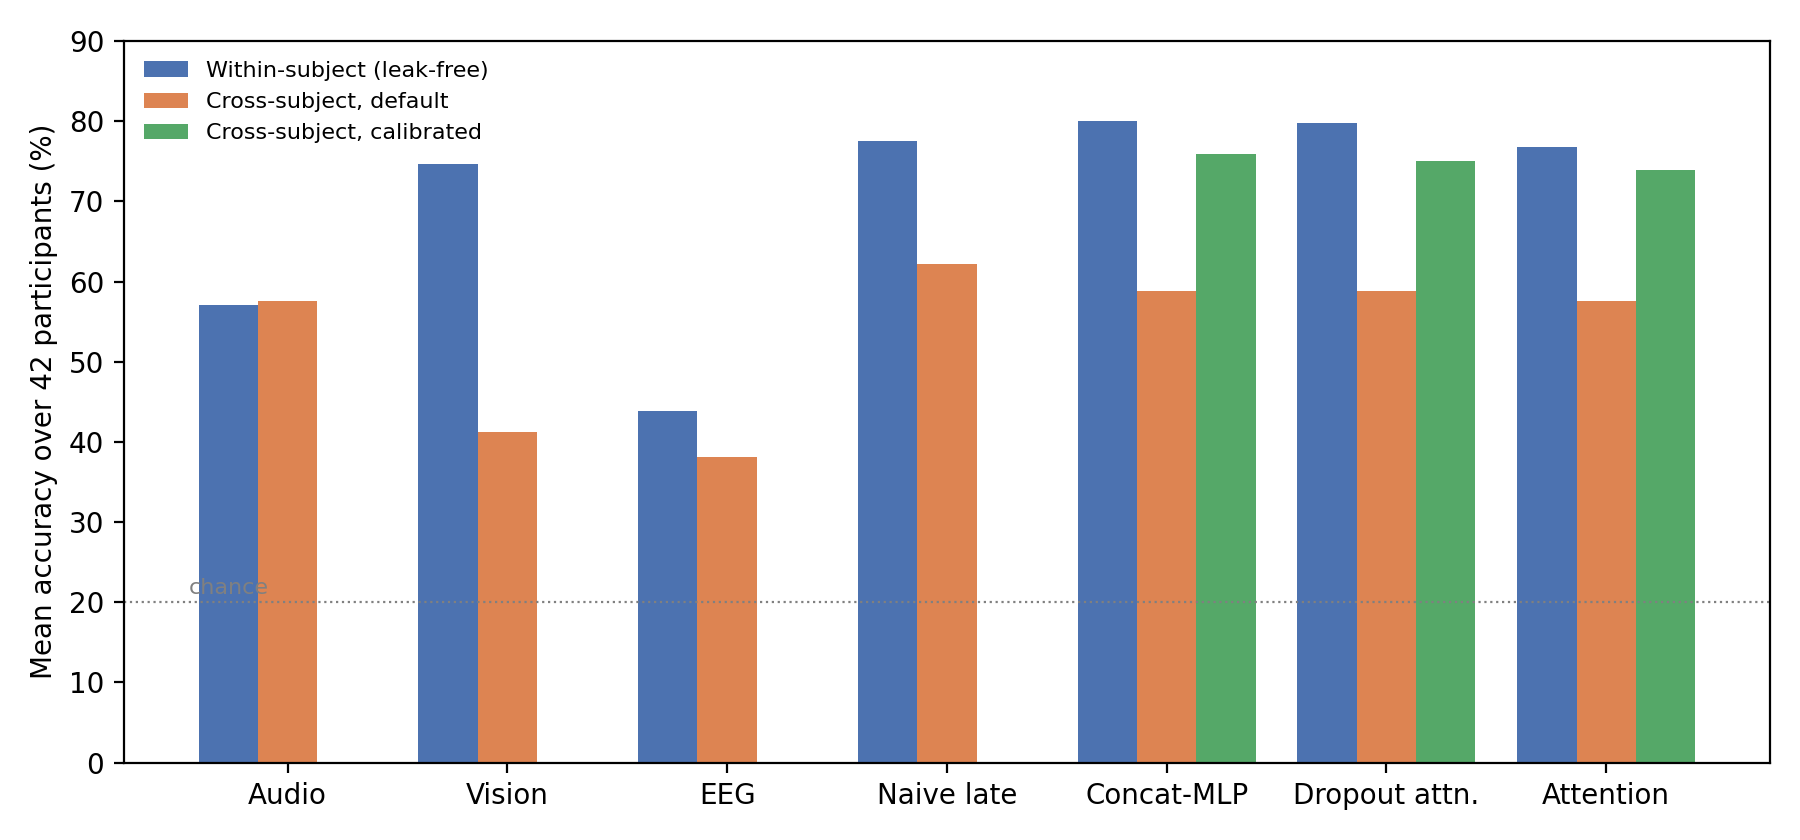
\includegraphics[width=\textwidth]{images/fig_within_cross.png}}{\fbox{\parbox{0.9\textwidth}{\centering Missing image placeholder: \texttt{images/fig\_within\_cross.png} (run \texttt{make\_p3\_figures.py}).}}}
\caption{Mean accuracy over 42 participants under the three protocols. Within-subject fusion figures are leak-free. Calibration (Chapter~\ref{chap:calibration}) acts only on the learned heads' inputs, so no calibrated bar is shown for the unimodal classifiers or naive late fusion.}
\label{fig:within_cross}
\end{figure}

The ordering of modalities inverts (Figure~\ref{fig:within_cross}). Within-subject, vision (74.6\%) $>$ audio (57.1\%)
$>$ EEG (43.9\%); cross-subject, audio (57.5\%) $>$ vision (41.2\%) $>$ EEG (38.2\%).
Audio, not vision, is the strongest single modality on unseen participants, and the
margin is large and highly significant ($+16.33$ pp, $p < 0.0001$).

A supplementary observation reinforces the interpretation. During calibration, the
vision encoder was trained under two budgets: the P2-matched 3~frozen $+$
2~fine-tuning epochs, and a reduced 1$+$1 schedule. Training the vision encoder
\emph{longer} produced \emph{worse} cross-subject accuracy (41.9\% against 45.8\% on
fold 0, $p = 0.031$), while the same additional training is beneficial within-subject.
Additional gradient steps on the training participants' faces actively degrade
performance on new faces.

\section{Discussion}
\label{sec:cs_discussion}

\subsection{Identity Inflation in Facial-Emotion Recognition on EAV}

The asymmetry between audio ($+0.4$ pp) and vision ($-33.4$ pp) admits a direct
interpretation: a substantial portion of EAV's within-subject vision accuracy
reflects participant identity rather than emotional expression.

Facial appearance is strongly identity-bound. When training and test trials come from
the same individual, a ViT can reduce its loss by associating specific facial
configurations---this person's particular smile, brow geometry, or resting
expression---with emotion labels. Such a model performs excellently on that individual
and poorly on anyone else. The finding that additional vision training degrades
cross-subject accuracy supports this reading: if the drop reflected underfitting, more
training would help; instead it hurts, which is the expected signature of an encoder
fitting participant-specific structure.

Chapter~\ref{chap:calibration} tests this interpretation directly
(Section~\ref{sec:cal_mechanism}). A linear probe identifies which of the 42
participants a trial came from with 100.0\% accuracy from the vision features, and
removing each participant's feature offset raises cross-subject emotion decoding from
vision by 13.6 points---more than for any other modality. The same probe also
decodes identity from audio at 97.0\%, so identity being \emph{present} is not what
distinguishes vision; what distinguishes it is how strongly its emotion decision
depends on identity.

This reframes the 74.6\% vision figure of Chapter~\ref{chap:within}. That number is
correct as measured, but it describes a participant-specialised model, not evidence
that facial-emotion features on EAV generalise. The implication extends beyond this
thesis: any within-subject vision result on EAV, including those of prior published
work on this benchmark, is subject to the same inflation.

\subsection{Why Learned Fusion Loses Under Subject Shift}

An earlier version of this analysis proposed that learned fusion heads lose because
they learn a modality-reliability prior from the training participants---weighting
vision heavily because vision is strong on them---and that this prior is wrong for a
new participant. The evidence of Chapter~\ref{chap:calibration} does not support that
account. Per-trial dynamic reweighting, which has no fitted prior, also loses to naive
averaging (Section~\ref{sec:cal_negative}); and per-participant feature normalisation,
which changes no weighting at all, lifts the same heads 15.7--17.1 points to well above
averaging.

The account the evidence does support concerns the input rather than the weighting. A
learned head receives features in which every participant occupies a characteristic
offset, and it is fitted on training participants whose offsets it can partly exploit.
A held-out participant's offset is new, so their features lie off the training
distribution in a direction that carries no emotional information. Naive late fusion
combines class probabilities rather than features, contains no fitted quantity that
the offset can mislead, and therefore degrades least. Its advantage here is robustness,
not expressiveness, and it disappears once the offset is removed.

This is a protocol-dependent conclusion, not a verdict on attention-based fusion.
With participant identity in the features, learned fusion loses to averaging on unseen
participants; with it removed, every learned head wins by 11 to 14 points. Both
statements are true, and reporting only one would misrepresent the system.

\subsection{The Magnitude of the Overall Drop}

The best leak-free within-subject system (concat-MLP, 79.96\%) falls to 62.2\% under
subject-independent evaluation with default normalisation (naive late fusion), a gap
of 17.8 points. This is the quantity that within-subject evaluation concealed. With
per-participant calibration the best cross-subject figure rises to 75.9\%
(Chapter~\ref{chap:calibration}), reducing the gap to 4.0 points.

The gap should not be read as a defect of the method. It is a property of the
evaluation protocol, and an equivalent gap is expected to exist---though it has not
been measured---for the prior published methods on this benchmark, all of which report
within-subject figures. What the present evaluation contributes is the measurement
itself, together with a localisation of where the loss originates.

What did \emph{not} degrade is the spread of individual difficulty. For naive late
fusion, the per-participant standard deviation is 0.093 cross-subject against 0.091
within-subject. The level moves; the shape of the population distribution does not.

\subsection{Robustness Under Missing EEG}

The zero-EEG configuration retains its practical viability. Under default
normalisation, modality-dropout fusion scores 58.77\% at full modality and 57.89\% with
EEG zeroed---a difference of 0.89 percentage points that is not statistically
significant ($p = 0.090$). The demonstration path, which operates without an EEG
headset, therefore degrades gracefully on unseen participants as well as on seen ones.

The corollary was initially read as unfavourable to the trimodal premise: if removing
EEG costs under one point, EEG adds little to the fused prediction on unseen
participants. Calibration changes this. With per-participant normalisation, removing
EEG costs 1.45 points and the loss is significant (Section~\ref{sec:cal_ranking}): EEG
contributes measurably once the representation stops encoding identity, though it
remains the smallest of the three contributions.

\section{Answers to Research Questions}
\label{sec:cs_rq}

\textbf{RQ6---Cross-subject generalisation:} The system generalises to unseen
participants at 62.2\% mean accuracy (naive late fusion, default normalisation),
substantially above the 20\% chance level but 15.3 percentage points below the same
method within-subject and 17.8 points below the best leak-free within-subject
configuration. All per-modality and fusion methods remain above chance on every fold.
The loss is concentrated in vision ($-33.4$ points) and is traced to participant
identity in Chapter~\ref{chap:calibration}, where per-participant calibration raises
the best cross-subject figure to 75.9\%.

\textbf{RQ7---Protocol dependence of the architectural contribution:} It depends on
the representation, not only on the protocol. Under subject-independent evaluation
with default normalisation, no learned fusion head outperforms naive softmax
averaging, and all three are 3.4--4.5 points worse and indistinguishable from one
another. With per-participant calibration, every learned head outperforms averaging by
11--14 points and the heads separate significantly (concat-MLP $>$ modality dropout $>$
cross-attention; Chapter~\ref{chap:calibration}). Within-subject, where both effects
are absent, learned fusion is at best marginally better than averaging.
